\documentclass[10.5pt]{proc}
\usepackage[T1]{fontenc}
\usepackage{graphicx}
\usepackage{hyperref}
\usepackage[small]{titlesec}
\usepackage{fontspec}
\usepackage{multirow}

\setmainfont{Times}
\setlength{\oddsidemargin}{0in}
\setlength{\textwidth}{16cm}
\setlength{\topmargin}{0in}
\setlength{\textheight}{8in}

\begin{document}
\title{Detecting Type of Tennis Shots from Broadcast Video\\[5pt]
\small{91.423/523 Computer Vision Final Project, UMass Lowell}}
\author{Kunal Vyas, Eugene Stanley\\
  \texttt{kunal\_vyas@student.uml.edu,}
  %\and
  \texttt{eugene\_stanley@student.uml.edu}}
  \date{\vspace{-1ex}}
  \maketitle
  
  \textbf{\large{Abstract}}\\[3pt]
  \emph{\normalsize{We have created an application which attempts to determine the type of shot hit by a lawn tennis player. There can be many different approaches to this. We discuss different methods that we tried by using basic OpenCV functions. In this article, we measure what novel approaches we followed, their performance and accuracy and the factors affecting them.}}
  \section{Introduction:}
  Watching professional tennis players play is the most important and fundamental way to improve one's own game. By observing certain statistics like the kind of shots hit during a tennis match, people can learn from what the professionals do and improve their own game.\\
      Shots could be classified by type so that they can be indexed and retrieved later for studying a particular shot technique. Video archives or old tennis matches could be data mined to provide a novice examples of the requested shot. Our goal is to create an application which can accurately and quickly categorize shots by various type.\\
  Our program takes in a video of a tennis match, and attempts to determine the type of shot hit by the player. The application will take broadcast video as input and output the type of shot being performed for each successful hit.\\[4pt]
    \begin{figure}[h]
    \centering
	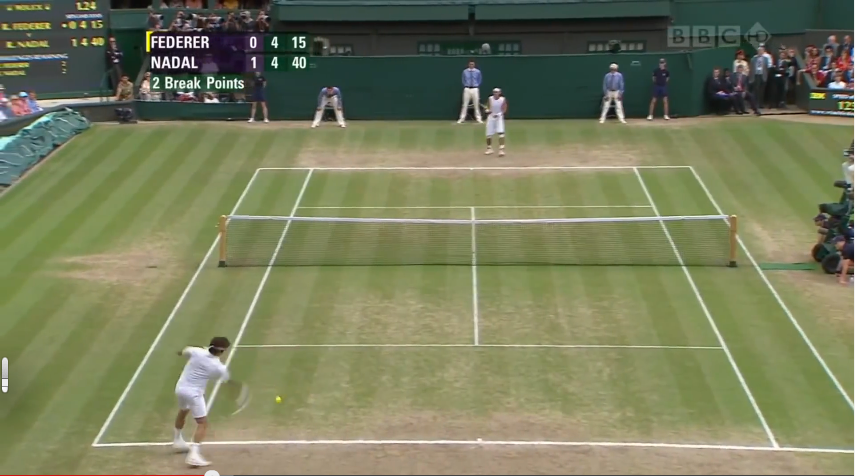
\includegraphics[width=.47\textwidth]{forehand.png}
	\caption{A screenshot of a sample input video}
	\end{figure}
    The motivation for this project comes from the need of match statistics which are often displayed after the matches. We think it is important to gather as many facts as possible because they can help in analysis and allow for degrees of improvement by learning from mistakes.\\
	Although implementations exist that are detecting activity of players, we have followed a different approach towards this problem. We have explored and used OpenCV's inbuilt functions and unlike other existing approaches, we are not using machine learning to solve this problem.
    
    \section{Background:}
    There are existing implementations that acheive the same goal:
    \subsection{CS229: Action Recognition in Tennis\cite{stanford2012}}
        This method was developed by Aman Sikka and Rajbir Kataria at Stanford University in 2012. It learns the three Tennis actions by using Support Vector Machines (SVMs) classifier. Accuracy is inconsistent and so we planned to get better results from our method.
    \subsection{Player Action Recognition in Broadcast Tennis Video with Applications to Semantic Analysis of Sports Game\cite{asians}}
    This method was developed by Guangyu Zhu, Changsheng Xu, Qingming Huang, Wen Gao and Liyuan Xing in 2006. It considers the mapping relationship between relative movements of different body parts and the regions in the image plane.
    \subsection{Action Recognition in Tennis Videos using Optical Flow and Conditional Random Fields\cite{argentina}}
    This proposed approach combines the application of video processing techniques for region of interest detection and feature extraction in tennis videos, and CRFs for action recognition.\\
    \\

    \section{Approach:}
	Our idea is to detect the player and ball and then use their positions to determine the actions performed. We used pre-trained haar cascades and consecutive frame subtraction to detect motion between frames.\\
	The player detection method gives us a rectangle and using it, we are learning about the position of the player on the court. For this to detect only the player we want, which is the one nearer to us, we are bounding the region of interest and working with that beyond that point. This also improves performance slightly. The accuracy of the application relies heavily on the accuracy of this detection.\\
	For ball detection, we are subtracting frames and finding the circles in the subtracted image. Like for player detection, we are doing this for a region of interest which is rectangular in shape.\\
    \begin{figure}[h]
    \centering
	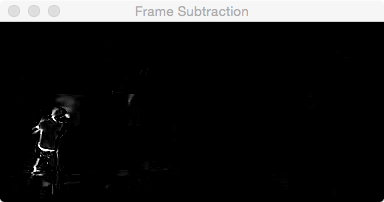
\includegraphics[width=.47\textwidth]{hough.png}\\
	\caption{Frame Subtraction}
	\end{figure}
	It would've been great if we could isolate the ball uniquely. But unfortunately, there were movements by players and that also showed up in the ball detection results.\\
	So we used a ball prediction approach to calculate where the ball is going to be just around when the player hits the ball. For this, we used only the minimum value of all the hough points. By knowing the direction of ball, i.e if it is coming towards the player or going away, we calculate the slope of the ball movement and predict the position of the ball continuously till it reaches the player. Then by knowing the x-positions of the player and the ball, we determine if the shot was hit from the right or left of the player. Considering the player is right handed, if the ball is hit from his/her right, it is a forehand, and a backhand otherwise.\\
	
	Our project can be found at \href{https://github.com/kv-kunalvyas/tennis}{\texttt{GitHub}}.\\
	
	\begin{table}[h]
	\caption{Summary of Submitted Code:}
	\begin{tabular}{|l|l|l|}
	\hline
	\textbf{filename} & \textbf{description}                                                    & \textbf{author} \\ \hline
	main.cpp          & \begin{tabular}[c]{@{}l@{}}Ball detection and\\ prediction\end{tabular} & Eugene Stanley  \\ \hline
	main.cpp          & \begin{tabular}[c]{@{}l@{}}Finding player's\\ position\end{tabular}     & Kunal Vyas      \\ \hline
	\end{tabular}
	\end{table}
	
    \section{Dataset:}
    For player detection, we used an upper body haar cascade detector from OpenCV's gihub repository. This is an xml file available on Opencv's Github repository.
    
    \section{Evaluation:}
	\subsection{Person Detection:}
    When we started with the project, we had decided to use the HoG Descriptor for person detection. We were getting wrong results. Later, we figured out that the reason for this was that the training sets for the person detection were not trained with what we were trying to solve. Tennis players especially when hitting shots, faced sideways and with their rackets in hand were not being detected. Also, the frame rate of the video dropped to 10 frames per second, and sometimes even lesser. We tried our program on people walking on a street and it was highly accurate with no loss of frames.\\
	We were looking for alternatives and we found a slighlty better way of doing the task. We used Haar-based Detectors For Pedestrian Detection\cite{cascade}. We used it to detect only the upper body of the people and this resulted in better accuracy. But still, for the most part, we have to change the values in the \texttt{detectMultiScale} function for it to recognize the players and the frame rate is still dropping.\\
	\subsection{Ball Detection:}
	We are using Hough Circles for detecting the ball. This method is giving us points for every moving object between frames. So when we run this detection approach, we are getting points for players as well as the moving ball.\\
	We devised a workaround for this. First, we neglect detections if the number is larger than 10. This happens when the camera is moving or the scene is changing. Secondly, we find the minimum value of y-coordinate among these, which is the farthest detected point from the player. This ensures that the ball is detected and it is the only one point that is being detected till it reaches the player.\\
	Then, we calculate if the ball is travelling towards or away from the player. Based on the slope of the ball which is travelling towards the player, and by taking the middle point of the rectangle where player was last detected, we decide if the shot hit was a forehand or a backhand.\\
	
	
	
	\subsection{Comparison:}
	The accuracy of this program varies hugely and depends on many factors like quality of video, movement and position of camera in the video, player getting detected properly, etc. However, running this for some videos gave us the following results:
	\begin{table}[h]
	\caption{Summary of approximate accuracy results:}
	\begin{tabular}{ll|c|c|}
	\cline{3-4}
	                                              &          & \multicolumn{2}{c|}{Predicted}                                \\ \cline{3-4} 
	                                              &          & \multicolumn{1}{l|}{Forehand} & \multicolumn{1}{l|}{Backhand} \\ \hline
	\multicolumn{1}{|c|}{\multirow{2}{*}{Actual}} & Forehand & 30\%                          & 70\%                          \\ \cline{2-4} 
	\multicolumn{1}{|c|}{}                        & Backhand & 10\%                          & 90\%                          \\ \hline
	\end{tabular}
	\end{table}

	Comparing this accuracy to the approach followed by \emph{Aman Sikka and Rajbir Kataria}\cite{stanford2012}:
	\begin{table}[h]
	\caption{Confusion Matrix using RBF Kernel}
	\label{my-label}
	\begin{tabular}{ll|c|c|}
	\cline{3-4}
	                                              &          & \multicolumn{2}{c|}{Predicted}                                \\ \cline{3-4} 
	                                              &          & \multicolumn{1}{l|}{Forehand} & \multicolumn{1}{l|}{Backhand} \\ \hline
	\multicolumn{1}{|c|}{\multirow{2}{*}{Actual}} & Forehand & 66.66\%                          & 0\%                          \\ \cline{2-4} 
	\multicolumn{1}{|c|}{}                        & Backhand & 0\%                          & 100\%                          \\ \hline
	\end{tabular}
	\end{table}

	Comparing these values, we see that our approach has a lot of false detections. This is firstly because we do not have a good method to detect the player. Secondly, when we are calculating the slope and then the type of shot using the last two points, one of those points is on the player's head, which drastically changes the slope and hence the ambiguity in results.

	\subsection{Alternate Approaches:}
	As we were finding a way to solve our problem, we thought about ways that we ultimately didn't use in the project.\\
	One such approach was to use just the points from the Hough Circles and then using maximum and average of x-coordinate detected values to determine the shot. This had limitations, because it wasn't capable of detecting for all scenarios.\\
	Other way our idea can be improved is by using a machine learning method to train sample of tennis players hitting the shots, because that is where our program performs poorly. Infact, sideways faces is one of the limitations of the player detection approach we have followed.\\
	We also tried to track the detected player positions using Lucas Kanade method for optical flow. But that failed too because it didn't track all points successfully and hence it was not reliable enough.\\
	There are many more improvements and ideas that we can implement to make the performance and accuracy better, but given the circumstances, we were not able to incorporate in this project.\\
	\subsection{Performance:}
    \begin{figure}[h]
    \centering
	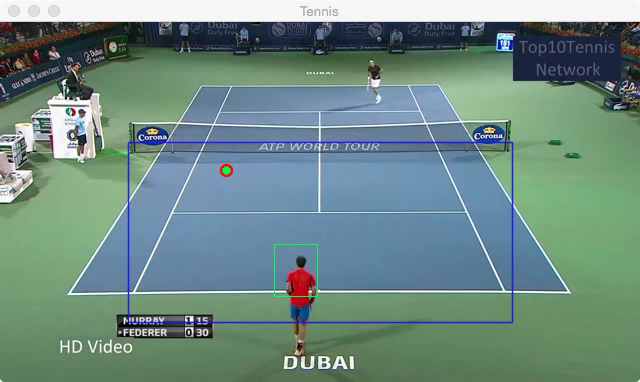
\includegraphics[width=.47\textwidth]{right.png}\\
	\caption{Successful result}
	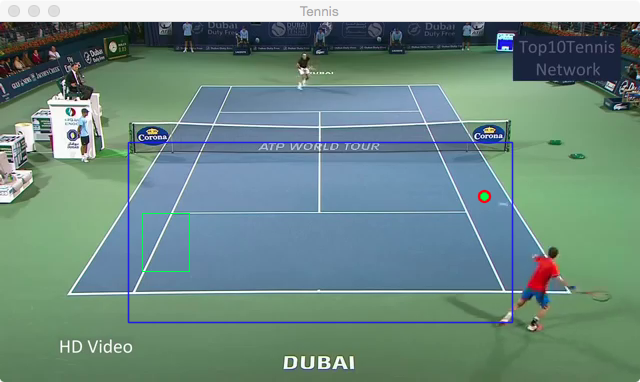
\includegraphics[width=.47\textwidth]{failure.png}\\
	\caption{Failed Result}
	\end{figure}
	
	\section{Conclusion:}
	We have concluded that our method has some shortcomings that can be overcome by learning techniques. The accuracy we got in the end are lesser than what we expected when we started the project.\\
	Detecting the player turns out to be a computationally expensive task, and that too with low accuracy.\\
	Settings have to be changed for each video because the detector has to be customized for the video. Also, the region of interest rectangle is not perfect for all videos, because of change in camera positions at different courts.\\
	For one of the videos, there was a shadow on the court and that caused disturbances in ball detection.\\
	\section{Team Roles:}
	\subsection{Kunal Vyas:}
	- Player detection.\\
	- Algorithm(discussed together).\\
	- Dataset collection.\\
	- Gathering results.\\
	- Lines of code written = ~100\\
	
	\subsection{Eugene Stanley:}
	- Ball detection\\
	- Algorithm(discussed together).\\
	- Major implementation of the ball algorithm\\
	- Testing\\
	- Lines of code written = ~175\\
	
	\newpage
\begin{thebibliography}{99}
	
\bibitem{hog}
OpenCV Object Detection. \\
\href{http://docs.opencv.org/modules/gpu/doc/object\_detection.html}{\emph{link}}

\bibitem{stanford2012}
Aman Sikka, Rajbir Kataria (2012) CS229: Action Recognition in Tennis, Stanford University, Stanford, CA -- 94305.\\
\href{http://cs229.stanford.edu/proj2012/KatariaSikka-ActionRecognitionInTennis.pdf}{\emph{link}}

\bibitem{asians}
Guangyu Zhu, Changsheng Xu, Qingming Huang, Wen Gao and Liyuan Xing (2006). Player Action Recognition in Broadcast Tennis Video with Applications to Semantic Analysis of Sports Game. 

\bibitem{argentina}
Jo\'se F. Manera, Jonathan Vainstein,Claudio Delrieux and Ana Maguitman (2013). Action Recognition in Tennis Videos using Optical Flow and Conditional Random Fields.
\href{http://42jaiio.sadio.org.ar/proceedings/simposios/Trabajos/AST/14.pdf}{\emph{link}}


\bibitem{cascade}
\href{https://github.com/Itseez/opencv/blob/master/data/haarcascades/haarcascade_upperbody.xml}{Github : Haar based detection for upper body detection}




\end{thebibliography}

\end{document} 